\documentclass[journal,12pt,twocolumn]{IEEEtran}

\usepackage{setspace}
\usepackage{gensymb}
\singlespacing
\usepackage[cmex10]{amsmath}

\usepackage{amsthm}

\usepackage{mathrsfs}
\usepackage{txfonts}
\usepackage{stfloats}
\usepackage{bm}
\usepackage{cite}
\usepackage{cases}
\usepackage{subfig}

\usepackage{longtable}
\usepackage{multirow}

\usepackage{enumitem}
\usepackage{mathtools}
\usepackage{steinmetz}
\usepackage{tikz}
\usepackage{circuitikz}
\usepackage{verbatim}
\usepackage{tfrupee}
\usepackage[breaklinks=true]{hyperref}
\usepackage{graphicx}
\usepackage{tkz-euclide}
\usepackage{textcomp}

\usetikzlibrary{calc,math}
\usepackage{listings}
    \usepackage{color}                                            %%
    \usepackage{array}                                            %%
    \usepackage{longtable}                                        %%
    \usepackage{calc}                                             %%
    \usepackage{multirow}                                         %%
    \usepackage{hhline}                                           %%
    \usepackage{ifthen}                                           %%
    \usepackage{lscape}     
\usepackage{multicol}
\usepackage{chngcntr}

\DeclareMathOperator*{\Res}{Res}

\renewcommand\thesection{\arabic{section}}
\renewcommand\thesubsection{\thesection.\arabic{subsection}}
\renewcommand\thesubsubsection{\thesubsection.\arabic{subsubsection}}

\renewcommand\thesectiondis{\arabic{section}}
\renewcommand\thesubsectiondis{\thesectiondis.\arabic{subsection}}
\renewcommand\thesubsubsectiondis{\thesubsectiondis.\arabic{subsubsection}}


\hyphenation{op-tical net-works semi-conduc-tor}
\def\inputGnumericTable{}                                 %%

\lstset{
%language=C,
frame=single, 
breaklines=true,
columns=fullflexible
}
\begin{document}


\newtheorem{theorem}{Theorem}[section]
\newtheorem{problem}{Problem}
\newtheorem{proposition}{Proposition}[section]
\newtheorem{lemma}{Lemma}[section]
\newtheorem{corollary}[theorem]{Corollary}
\newtheorem{example}{Example}[section]
\newtheorem{definition}[problem]{Definition}

\newcommand{\BEQA}{\begin{eqnarray}}
\newcommand{\EEQA}{\end{eqnarray}}
\newcommand{\define}{\stackrel{\triangle}{=}}
\bibliographystyle{IEEEtran}
\raggedbottom
\setlength{\parindent}{0pt}
\providecommand{\mbf}{\mathbf}
\providecommand{\pr}[1]{\ensuremath{\Pr\left(#1\right)}}
\providecommand{\qfunc}[1]{\ensuremath{Q\left(#1\right)}}
\providecommand{\sbrak}[1]{\ensuremath{{}\left[#1\right]}}
\providecommand{\lsbrak}[1]{\ensuremath{{}\left[#1\right.}}
\providecommand{\rsbrak}[1]{\ensuremath{{}\left.#1\right]}}
\providecommand{\brak}[1]{\ensuremath{\left(#1\right)}}
\providecommand{\lbrak}[1]{\ensuremath{\left(#1\right.}}
\providecommand{\rbrak}[1]{\ensuremath{\left.#1\right)}}
\providecommand{\cbrak}[1]{\ensuremath{\left\{#1\right\}}}
\providecommand{\lcbrak}[1]{\ensuremath{\left\{#1\right.}}
\providecommand{\rcbrak}[1]{\ensuremath{\left.#1\right\}}}
\theoremstyle{remark}
\newtheorem{rem}{Remark}
\newcommand{\sgn}{\mathop{\mathrm{sgn}}}
\providecommand{\abs}[1]{\left\vert#1\right\vert}
\providecommand{\res}[1]{\Res\displaylimits_{#1}} 
\providecommand{\norm}[1]{\left\lVert#1\right\rVert}
%\providecommand{\norm}[1]{\lVert#1\rVert}
\providecommand{\mtx}[1]{\mathbf{#1}}
\providecommand{\mean}[1]{E\left[ #1 \right]}
\providecommand{\fourier}{\overset{\mathcal{F}}{ \rightleftharpoons}}
%\providecommand{\hilbert}{\overset{\mathcal{H}}{ \rightleftharpoons}}
\providecommand{\system}{\overset{\mathcal{H}}{ \longleftrightarrow}}
	%\newcommand{\solution}[2]{\textbf{Solution:}{#1}}
\newcommand{\solution}{\noindent \textbf{Solution: }}
\newcommand{\cosec}{\,\text{cosec}\,}
\providecommand{\dec}[2]{\ensuremath{\overset{#1}{\underset{#2}{\gtrless}}}}
\newcommand{\myvec}[1]{\ensuremath{\begin{pmatrix}#1\end{pmatrix}}}
\newcommand{\mydet}[1]{\ensuremath{\begin{vmatrix}#1\end{vmatrix}}}
\numberwithin{equation}{subsection}
\makeatletter
\@addtoreset{figure}{problem}
\makeatother
\let\StandardTheFigure\thefigure
\let\vec\mathbf
\renewcommand{\thefigure}{\theproblem}
\def\putbox#1#2#3{\makebox[0in][l]{\makebox[#1][l]{}\raisebox{\baselineskip}[0in][0in]{\raisebox{#2}[0in][0in]{#3}}}}
     \def\rightbox#1{\makebox[0in][r]{#1}}
     \def\centbox#1{\makebox[0in]{#1}}
     \def\topbox#1{\raisebox{-\baselineskip}[0in][0in]{#1}}
     \def\midbox#1{\raisebox{-0.5\baselineskip}[0in][0in]{#1}}
\vspace{3cm}
\title{Assignment 6}
\author{Gautham Bellamkonda - CS20BTECH11017}
\maketitle
\newpage
\bigskip
\renewcommand{\thefigure}{\theenumi}
\renewcommand{\thetable}{\theenumi}
Download all
%\begin{lstlisting}
%https://github.com/GauthamBellamkonda/AI1103/tree/main/Assignment6/Codes
%\end{lstlisting} 
latex-tikz codes from 
\begin{lstlisting}
https://github.com/GauthamBellamkonda/AI1103/tree/main/Assignment6
\end{lstlisting}
\section{Problem}
Let $X_1, X_2, \ldots , X_n$ be a random sample of size $n \; ( \geq 2 ) $ from a distribution having the probability density function
\begin{align}
f(x;\theta) = 
\begin{cases}
\dfrac{1}{\theta} \exp\brak{-\dfrac{x}{\theta}} & x > 0, \\
0, & \text{otherwise,}
\end{cases}
\end{align}
where $\theta \in (0, \infty)$. Let $X_{(1)} = $ min $ \{ X_1, X_2, \ldots , X_n \} $ and $T = \sum_{i=1}^n X_i $. Then $E(X_{(1)} | T)$ equals $\ldots \ldots \ldots$
\begin{enumerate}[label = (\Alph*)]
\item $\dfrac{T}{n^2}$ \\
\item $\dfrac{T}{n}$ \\
\item $\dfrac{(n+1)T}{2n}$ \\
\item $\dfrac{(n+1)^2 T}{4n^2}$
\end{enumerate}

\section{Prerequisites}
\begin{lemma}[Sum of Gamma random variables]
Suppose that $X_1, X_2, X_3, \ldots X_n$ are $n$ gamma variables with parameters $k$ and $\theta$, $X_i \sim \Gamma(k, \theta)$. Then the sum $T = \sum_{i=1}^{n} X_i$ follows a gamma distribution with parameters $nk$ and $\theta$, $T \sim \Gamma(nk, \theta)$
\end{lemma}
\begin{definition}[Complete Statistic]
The statistic $T$ is said to be complete for the distribution of $X$ if, for every measurable function $g$, if
\begin{align}
E(g(T)) = 0 \; \forall \; \theta \Rightarrow \pr{g(T)=0} = 1 
\end{align}
\end{definition}
\begin{definition}[Sufficient Statistic]
A statistic $t = T(X)$ is sufficient for underlying parameter $\theta$ precisely if the conditional probability distribution of the data $X$, given the statistic $t = T(X)$, does not depend on the parameter $\theta$. 
\end{definition}
\begin{theorem}[Fischer-Neymann Factorisation theorem]
If the probability density function is $f_\theta (x)$, then $T$ is sufficient for $\theta$ if and only if nonnegative functions $g$ and $h$ can be found such that
\begin{align}
f_\theta (x) = h(x)g_\theta(T(x))
\end{align}
\end{theorem}
\begin{lemma} \label{lemma_sufficient_complete}
\begin{align}
T = \sum_{i=1}^{n} X_i
\end{align}
is a complete and sufficient statistic. 
\end{lemma}
\begin{proof}
\begin{enumerate}
\item \textit{(Sufficiency)}
\begin{align}
f_{X}(x_1, x_2, \ldots x_n) &= f_{X_1}(x_1)f_{X_2}(x_2) \ldots f_{X_n}(x_n)\\
&= \dfrac{1}{\theta} \exp\brak{-\dfrac{x_1}{\theta}} \cdots \dfrac{1}{\theta} \exp\brak{-\dfrac{x_n}{\theta}}\\
&= 1 \cdot \dfrac{1}{\theta^n} \exp\brak{-\dfrac{T}{\theta}}\\
&= h(X) \cdot g(T, \theta) 
\end{align}
with 
\begin{align}
g(T, \theta) &= \dfrac{1}{\theta^n} \exp\brak{-\dfrac{T}{\theta}}\\
h(X) &= 1
\end{align}
Therefore, $T$ is a sufficient statistic.\\
\item \textit{(Completeness)}\\
$X_i$ follow a gamma distribution, $X_i \sim \Gamma (1, \frac{1}{\theta})$. Hence, $T = \sum_{i=1}^n X_i $ follows a gamma distribution, $T \sim \Gamma (n, \frac{1}{\theta})$. Therefore, the expected value of a function $g$ is
\begin{align}
E(g(T)) &= 
\int_0 ^{\infty} g(t) \dfrac{t^{n-1} e^{-\frac{t}{\theta}}}{\theta^n(n-1)!} dt\\ 
&= \frac{1}{\theta^n (n-1)!} \int_0 ^{\infty} g(t) t^{n-1} e^{-\frac{t}{\theta}} dt\\ 
&= \frac{1}{\theta^n (n-1)!} F \brak{\frac{1}{\theta}}\\
&= 0 \text{ for all } \theta > 0.
\end{align}
where, 
\begin{align}
f(t) &= t^{n-1}g(t)\\
F \brak{\frac{1}{\theta}} &= \text{Laplace Transform of} f(t) \text{ at } \theta
\end{align}
Since, $E(g(T))=0$ for all $\theta > 0$, 
\begin{align}
\label{eqn}
F \brak{\frac{1}{\theta}} &= 0 \text{ for all } \theta > 0.
\end{align}
From the theory of Laplace transforms, it follows from \eqref{eqn} that
\begin{align}
f(t)=0 \text{ almost everywhere in } (0, \infty)\\
g(t)=0 \text{ almost everywhere in } (0, \infty)\\
\pr{g(t)=0} = 1
\end{align}

Therefore, $T$ is a complete statistic.
\end{enumerate}
\end{proof}
\begin{theorem}[Lehmann–Scheffé theorem]
If $T$ is a complete sufficient statistic for $\theta$ and 
\begin{align}
\label{eqn 2.0.1}
E(g(T)) = \tau(\theta)
\end{align}
then $g(T)$ is the uniformly minimum-variance unbiased estimator (UMVUE) of $\tau(\theta)$.
\end{theorem}
\section{Solution}
\begin{proposition} \label{prop_3.1}
$E(X_{(1)}|T)$ is the uniformly minimum-variance unbiased estimator (UMVUE) of $E(X_{(1)})$
\end{proposition}
\begin{proof}
By the law of total expectation, 
\begin{align}
\label{eqn 2.0.3}
E\brak{E(X_{(1)} | T )} = E(X_{(1)})
\end{align}
We know that $T = \sum_{i=1}^n X_i$ is a complete and sufficient statistic by \ref{lemma_sufficient_complete}. By Lehmann–Scheffé theorem, with
\begin{align}
\theta &= X_{(1)},\\ 
\tau(x) &= E(x),\\
g(T) &= E(X_{(1)} | T).
\end{align}
it follows from \eqref{eqn 2.0.3} that $E(X_{(1)} | T)$ is the UMVUE of $E(X_{(1)})$.
\end{proof}
\begin{proposition} \label{prop_3.2}
$\frac{T}{n^2}$ is uniformly minimum-variance unbiased estimator (UMVUE) of $E(X_{(1)})$
\end{proposition}
\begin{proof}
\begin{enumerate}
\item Let's find the probability distribution function and the expectation value of $X_{(1)}$ : 
\begin{align}
\pr{X_{(1)} > x} &= \pr{X_1 > x}\ldots \pr{X_n > x}\\
&= (1-F_{X_{1}}(x))\ldots(1-F_{X_{n}}(x))\\
&= (1-F_{X_{1}}(x))^n \\
&= \exp\brak{-\frac{nx}{\theta}}\\
F_{X_{(1)}}(x) &= 1 - \exp\brak{-\frac{nx}{\theta}}\\
f_{X_{(1)}}(x) &= \frac{n}{\theta} \exp\brak{-\frac{nx}{\theta}}
\end{align}
Therefore, $X_{(1)}$ follows an exponential distribution with mean $\dfrac{\theta}{n}$.
\begin{align}
E(X_{(1)}) = \frac{\theta}{n}
\end{align}
\item $\frac{T}{n^2}$ is uniformly minimum-variance unbiased estimator (UMVUE) of $E(X_{(1)})$, since $E\brak{\frac{T}{n^2}} = E(X_{(1)})$ : \\
Note that,
\begin{align}
E\brak{\frac{T}{n^2}} &= E\brak{\frac{\sum_{i=1}^n X_i}{n^2}}\\
&= \frac{E(\sum_{i=1}^n X_i)}{n^2}\\
&= \sum_{i=1}^n \frac{E(X_i)}{n^2}\\
&= \sum_{i=1}^n \frac{\theta}{n^2}\\
&= \frac{\theta}{n}\\
&= E(X_{(1)})
\end{align}
\end{enumerate}
Therefore, by Lehmann–Scheffé theorem, with
\begin{align}
\theta &= X_{(1)},\\
\tau(x) &= E(x),\\
g(T) &= \frac{T}{n^2},
\end{align}
it follows that $\dfrac{T}{n^2}$ is UMVUE of $E(X_{(1)})$.\\
\end{proof}
Since there exists a unique UMVUE for $E(X_{(1)})$, it follows from Proposition \ref{prop_3.1} and Proposition \ref{prop_3.2} that 
\begin{align}
E(X_{(1)} | T) = \frac{T}{n^2} 
\end{align}
Hence, option A is correct.
\begin{figure}[!hbt]
    \centering
	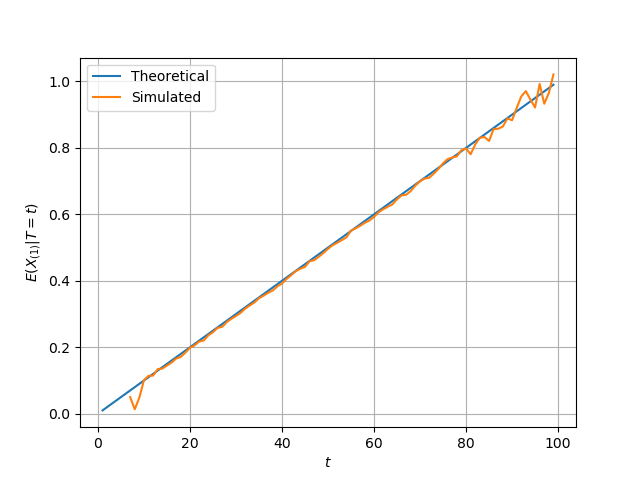
\includegraphics[width=\columnwidth]{./Figures/Figure_1.png}
    \caption{Theory vs Simulated plot of $E(X_{(1)} |T)$}
    \label{CDF_Y}
\end{figure}
\end{document}